\documentclass[12pt,letterpaper]{article}
\usepackage{comment} % enables the use of multi-line comments (\ifx \fi) 
\usepackage{mathtools}%%this is an extension to amsmath and corrects some glitches in that
\usepackage{mathrsfs}
\usepackage{ifpdf}
\usepackage{style}
\usepackage{float}


\begin{document}

\titlep{Wireless Indoor Localization through Machine Learning Techniques}{Owen McClure}{Intro to Data Mining and Machine Learning}{23 April, 2020}

\headr{McClure}

\frenchspacing\raggedright\setlength{\parindent}{.5in}
 
\sect{Introduction}


\par With the recent explosion is internet of things devices the need for a cheap and reliable method to determine the location of WiFi connected devices has become a very popular research topic. There are a few methods that can be used to determine the locations of internet connected devices, until recently one of the most popular methods would have been to use GPS. However, using GPS comes with a few problems. For one, it's signal is not very strong indoors and can even be non existent underground, another issue is that GPS is not normally precise enough to determine a location down to an individual room in a building. Another method to determine the location of WiFi connected devices is to use a the wireless signal strength itself. All devices connected to a wireless signal have a received signal strength indication or RSSI. Since wireless signal strength decays the farther a device is from its source (a WiFi router in this case) it should be possible the use the RSSI as a measure of the distance from a router. And with the signal strength measurements from multiple routers an actual location can be determined for the given device. 

\par The ability to determine the location of a WiFi connected device using nothing but it's surrounding networks has a wide variety of uses. One of the biggest applications that comes to mind is navigation through large networks of buildings, or for tracking foot-traffic in campuses. Other uses could be for emergency applications where the location of a person needs to be discovered quickly, or for smart buildings to track people's movement through them. However a potential drawback of all these applications is that an algorithm needs to be trained to locate devices in the specified locations for each individual application. A better approach to localization using WiFi would be triangulate a precise location rather than classify a location based on a room. 

\sect{Localization as a Classification Problem}

\par If locations are measured as individual rooms in a building, then this problem can be solved using a machine learning classification algorithm to classify a vector of signal strength measures as corresponding to a given room that a device is in. The data set for this topic is the Wireless Indoor Localization set taken from the University of California Irving data set repository. The set includes two-thousand observations of the RSSI of seven access points, with each observation followed by the room name (in this case a number from 1 to 4). The data is described as collected from an office building in Pittsburgh, USA. Since all seven RSSI are measured in the same units (dBm) it is not necessary to normalize or scale the data set for this problem. 
\begin{figure}[H]

  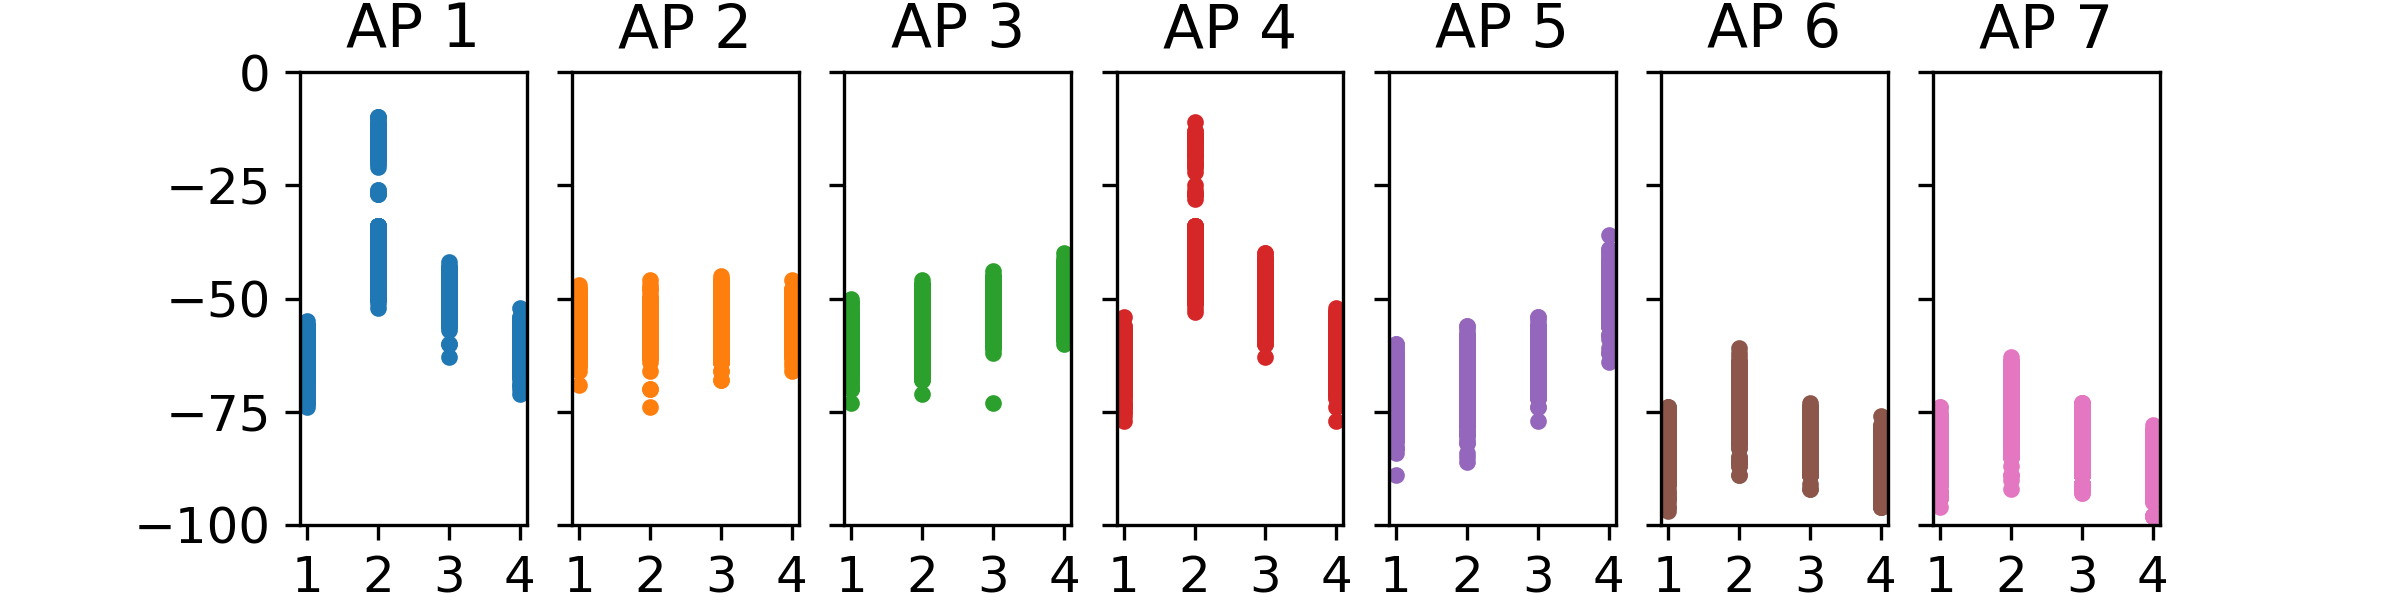
\includegraphics[width=170mm]{gph.png}
  \caption{Each AP's RSSI versus the room location}
  \label{fig:RSSI}

\end{figure}
\par Whats interesting about this data set is that based on Figure \ref{fig:RSSI} the location is not necessarily obvious just by looking at the signal from one access point, because of overlap with other rooms. However the classification algorithms will use data from all seven access points to determine the location. 

\par I also collected my own data from the WiFi networks around my house. The data collected is exactly the same a what is on the UCI website except it is taken across 5 rooms. This data set contains locations of rooms that are very close together (less than 5 feet apart) and so classification of locations for this set is not expected to be as accurate as the UCI data set. The rooms which I used are:
\begin{lstlisting}[basicstyle=\ttm\linespread{.8}\small]
    Room 1 = My Bedroom
    Room 2 = Entryway
    Room 3 = TV Room
    Room 4 = Kitchen
    Room 5 = Basement
\end{lstlisting}

\begin{figure}[H]

  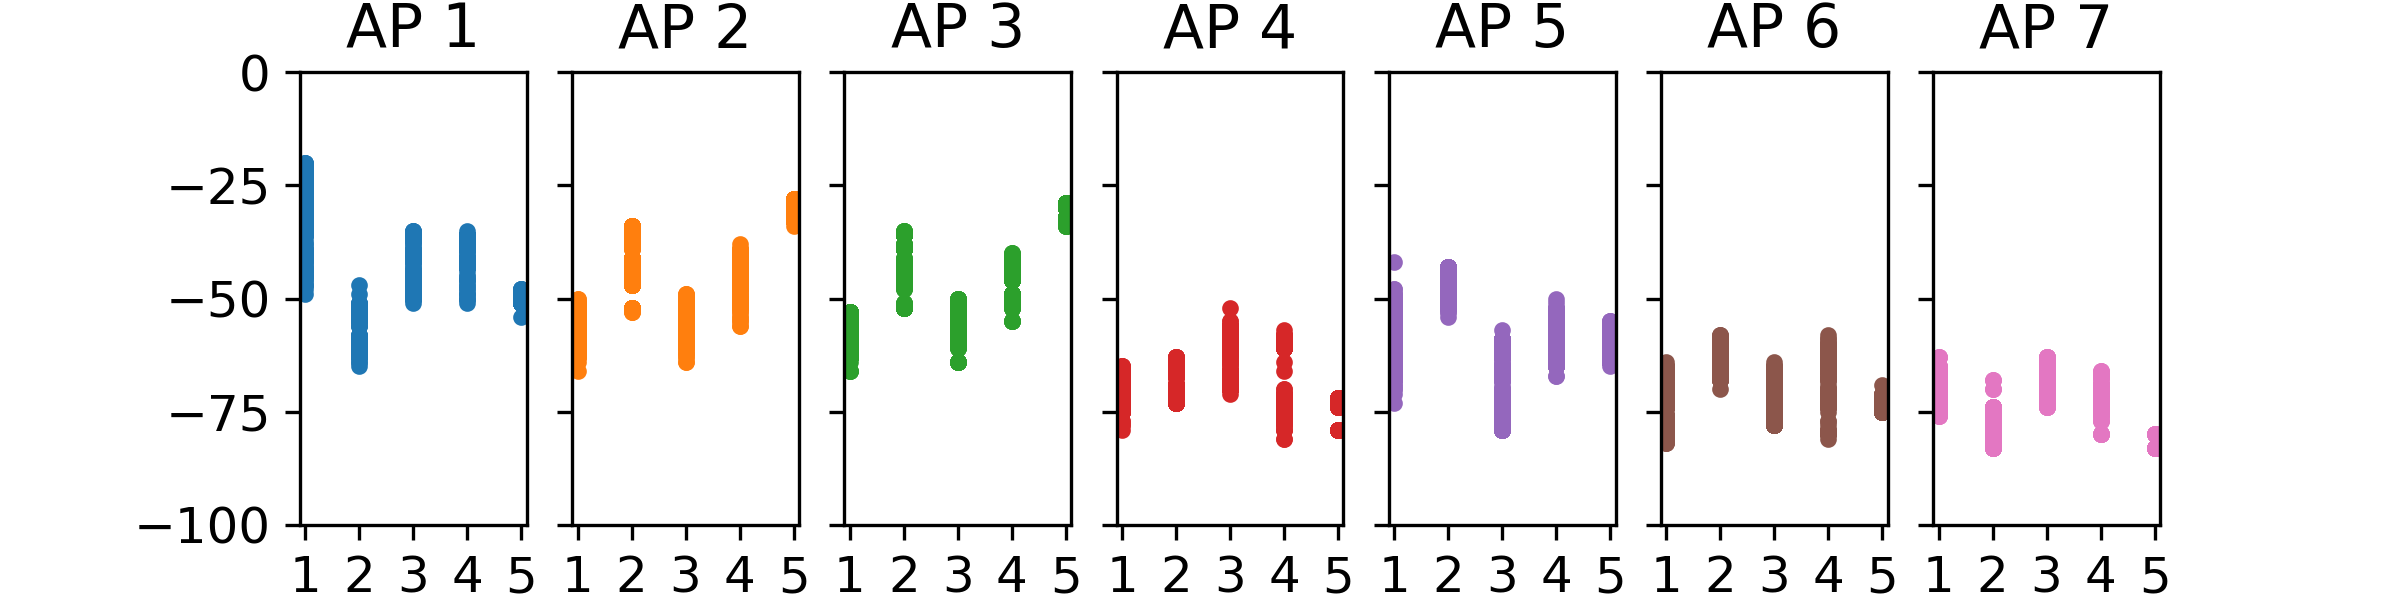
\includegraphics[width=170mm]{mygph.png}
  \caption{Each AP's RSSI versus the room in my house}
  \label{fig:myRSSI}

\end{figure}

\sect{SVM Classification}

For SVM classification the data was split into 67\% training data and 33\% testing data. Then the the SVM model from the sklearn module was used to build and classify a model. In order to choose a value for the regularization parameter an array of thirty values ranging from 1e-5 to 1000 was constructed and each one was used to fit the data. The value which produced the best score was then used as the regularization parameter. A similar process was used for an SVM with a linear kernel function, however it consistently performed worse than the Gaussian kernel function and so it is not included here.

\begin{python}
def svmReg(X_train, X_test, y_train, y_test):
    Cs = []
    scores_gau = []        
    for i in range(29):
        #I chose this because its a nice range from 1e-5 to 1000
        Cs.append(1e-5 * (1.75 ** i) )
    for c in Cs:
        model = svm.SVC( C=c, kernel = 'rbf' )
        model.fit(X_train, y_train)
        scores_gau.append(model.score(X_test, y_test))
    bestI_gau = np.argmax(scores_gau)
    print("\nSVM Results")
    print("Best testing C =", Cs[bestI_gau])
    print("Score =", scores_gau[bestI_gau]*100)
\end{python}

\par The resulting scores for both data sets when using the SVM classification model are both very high; the data set from UCI scores an average around 98.63\%. And the data collected in my own home scores even higher on average around 99.61\%. Both these classification scores are much better than what was expected, and their accuracy can most likely be attributed to the fact that this problem is being simplified as a classification problem of rooms.

\sect{KNN Classification}

\par Because of the nature of how a KNN model classifies data this set should be very accurate at determining locations. This is because intuitively vectors of signal strengths from the same room are expected to be similar to each other, and so would appear closer together as points. Again it's not necessary to scale x values because they are all measurements in the same units. For this problem both sets of data were cross validated using 5 fold cross validation, and the best k value was chosen to compute the score. Interestingly for both data sets and many different train/test splits the k value was almost always 3.

\begin{python}
def KNNReg(X_train, X_test, y_train, y_test):
    neighbor = [1, 3, 5, 7, 9]
    cv_score = []
    for k in range(0,5):
        knn_model=KNeighborsClassifier(n_neighbors=neighbor[k],
            p=2,metric='minkowski')
        score=cross_val_score(knn_model,X_train,y_train,cv=5,scoring='accuracy')
        cv_score.append(np.mean(score))
    best = np.argmax(cv_score)
    print("\nKNN Results")
    print("Best k =", neighbor[best])
    print("Score =", cv_score[best]*100)
\end{python}

\par For both datasets the scores were very good again with the UCI set scoring on average a 98.28\% and the data set from my house scoring 99.42\%. 

\sect{Further Thoughts}

\par The very high scores of both these data sets is pleasing to see, however as mentioned at the end of the SVM section the success of the classification is most likely due to the simplification of the problem. Although it makes sense and is much simpler to treat each room as a class and then to identify each RSSI vector as being in a particular room, there are a few disadvantages. In order to implement this method in a new environment data must be collected that can then be used to train the model, and if a new room is ever to be added to the model it must be re trained with more data from the additional room. This heavily limits the expansion and upgrading of this method which is not very ideal for commercial applications. To get around some of these drawbacks one solution is to classify a grid of points rather than individual rooms, this way a model does not have to be retrained every time a new room is added. This method would also allow for a much better picture of how a device moves through the given area over time, which would be helpful in tracking applications.

\par A much more versatile approach would be to use the input vector and some sort of regression to return another vector which would correspond to a location. This location vector could be either latitude and longitude, or x and y distances from a given point (really any coordinate system could work). Using a location vector rather than a room name is much more complicated to implement than classifying rooms, however it comes with distinct advantages. First of all if a coordinate system is chosen that is relative to an access point a new algorithm doesn't need to be trained when implementing localization in a new environment. Also since there is no room, or reference point constraint a location can take on a continuous value which would allow for more precision, and a much better degree of tracking objects over time.

\par One such method that implements localization in this way is Dr.Sharan Naribole's github repository where the locations of devices were predicted as latitude and longitude coordinates. Another paper; ``Machine Learning Algorithm for Wireless Indoor Localization'' uses a similar approach to Naribole although the latitude and longitude are not used but instead locations are mapped to a coordinate x and y plane. Whats different about both these projects from the classification method, is that there is much more attention paid to the signal integrity and how environmental interference may affect the accuracy of the model.

\par While the advantages described above may allow for a much more precise implementation of localization this may also act ad a disadvantage in some use cases. If its not necessary to be able to determine a location down to the nearest meter but instead all that's needed is a room location, then the classification method is a better choice, this is because its can be rapidly set up with very little attention paid to signal strength fluctuation, reflection, or interference due to walls or movement of people. Because of these reasons the data to train a new algorithm could be collected in as little as an hour with multiple devices, whereas to retrain a new non-classification model careful attention must be paid to signal fluctuations and interference.

\par In the future with more time it might be useful to explore methods which do not use classification but instead use regression to determine location. It would also be interesting to collect more data around my house and to refit the model for more rooms. Another aspect of this problem that could be explored is the minimum number of access points which can be used to still accurately determine a room location. Initially I wanted to collect the wireless data from inside RIT's campus and use that for classification, but in light of the virus outbreak this was not possible.

%=============================================

\begin{workscited}

\bibent
Abdullah, O. A., \& Abdel-Qader, I. (2018). Machine Learning Algorithm for Wireless Indoor Localization. \textit{Machine Learning - Advanced Techniques and Emerging Applications}. doi: 10.5772/intechopen.74754

\bibent
Rohra, J. G., Perumal, B., Narayanan, S. J., Thakur, P., \& Bhatt, R. B. (2017). User Localization in an Indoor Environment Using Fuzzy Hybrid of Particle Swarm Optimization \& Gravitational Search Algorithm with Neural Networks. \textit{Advances in Intelligent Systems and Computing Proceedings of Sixth International Conference on Soft Computing for Problem Solving}, 286–295. doi: 10.1007/978-981-10-3322-3\_27

\bibent
Naribole, Sharan, wlan\_localization, (2017), GitHub repository, \texttt{https://github.com/sharan-naribole/wlan\_localization}

\bibent
F. Zafari, A. Gkelias and K. K. Leung, "A Survey of Indoor Localization Systems and Technologies," \textit{IEEE Communications Surveys \& Tutorials}, vol. 21, no. 3, pp. 2568-2599, thirdquarter 2019.

\bibent
Zhang, G., Wang, P., Chen, H., \& Zhang, L. (2019). Wireless Indoor Localization Using Convolutional Neural Network and Gaussian Process Regression. \textit{Sensors, 19}(11), 2508. doi: 10.3390/s19112508

\end{workscited} 
%%\end{mla}
\end{document}


\ifx
Comments!
\fi